\chapter{\textbf{Materiales}}
\label{chapter:materiales}

\subsection*{Hardware}
\phantomsection
\addcontentsline{toc}{section}{Hardware}
\vspace{5mm}

Tal y como se menciona en la Introducción, el proyecto cuenta con un hardware específico (Figura \ref{fig:materials}, Raspberry Pi y cámara) que se entregará durante la primera sesión dedicada al trabajo. Su uso es obligatorio. 

En casos especiales donde el proyecto requiera algún elemento de hardware más complejo (impresión 3D, electrónica, etc.) se recomienda comunicarlo a los profesores lo antes posible (especialmente en el caso de impresión 3D, pues hay que consultar disponibilidad en la Universidad).

Por otro lado, desde el punto de vista de software, se puede hacer uso de cualquier librería, aunque el uso de modelos avanzados de Visión por Ordenador (Deep Learning) debe consultarse con los profesores ya que no es el objetivo de esta asignatura. Por último, también está disponible el uso de una Api Key de OpenAI para proyectos en los que pueda aportar valor.

\begin{figure}[H]
    \centering
    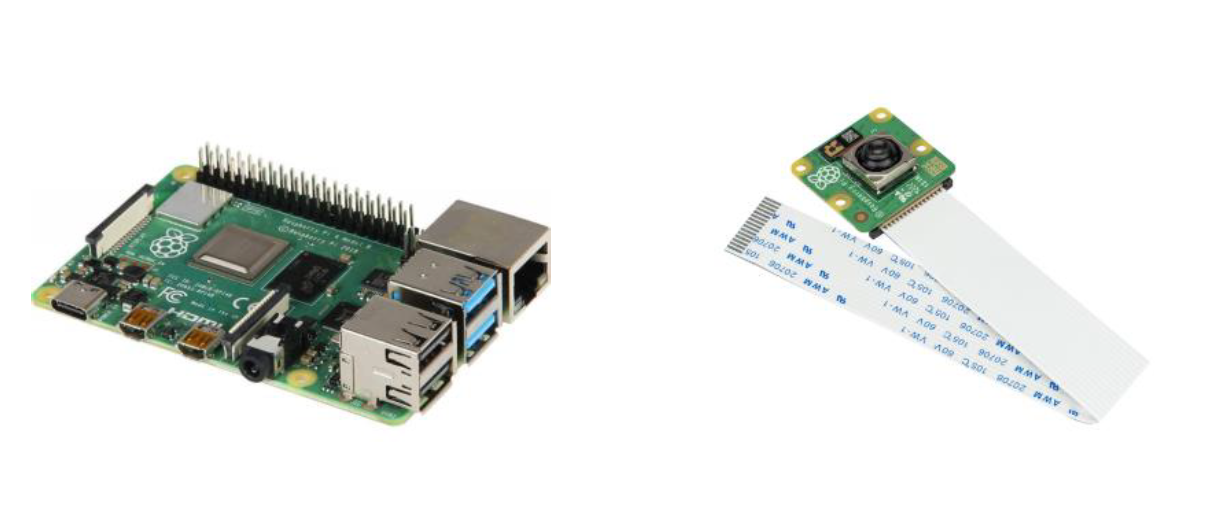
\includegraphics[width=0.65\textwidth]{Lab_Project/template/figures/materials.png}
    \caption{Materiales básicos pro porcionados: Raspberry Pi 4 y Cámara.}
    \label{fig:materials}
\end{figure}
